%% Template for SDP report, adapted from mlp_cw2_template, 2018. 

%% Based on  LaTeX template for ICML 2017 - example_paper.tex at 
%%  https://2017.icml.cc/Conferences/2017/StyleAuthorInstructions

\documentclass{article}
\usepackage[T1]{fontenc}
\usepackage{amssymb,amsmath}
\usepackage{txfonts}
\usepackage{microtype}
\usepackage{xspace}
\xspaceaddexceptions{\%}

% Lists with less spacing between items
\usepackage{paralist}

% For figures
\usepackage{graphicx}
\usepackage{subfig} 

% For citations
\usepackage{natbib}

% For algorithms
\usepackage{algorithm}
\usepackage{algorithmic}

% the hyperref package is used to produce hyperlinks in the
% resulting PDF.  If this breaks your system, please commend out the
% following usepackage line and replace \usepackage{mlp2017} with
% \usepackage[nohyperref]{mlp2017} below.
\usepackage{hyperref}
\usepackage{url}
\urlstyle{same}

% Packages hyperref and algorithmic misbehave sometimes.  We can fix
% this with the following command.
\newcommand{\theHalgorithm}{\arabic{algorithm}}


% Set up MLP coursework style (based on ICML style)
\usepackage{mlp2018}
\mlptitlerunning{SDP Demo \demoNumber  Group (\groupNumber)}
\bibliographystyle{icml2017}


\DeclareMathOperator{\softmax}{softmax}
\DeclareMathOperator{\sigmoid}{sigmoid}
\DeclareMathOperator{\sgn}{sgn}
\DeclareMathOperator{\relu}{relu}
\DeclareMathOperator{\lrelu}{lrelu}
\DeclareMathOperator{\elu}{elu}
\DeclareMathOperator{\selu}{selu}
\DeclareMathOperator{\maxout}{maxout}







%% You probably do not need to change anything above this comment

%% REPLACE the details in the following commands with your details
\setGroupNumber{20}
\setGroupName{ERNS}
\setProductName{FInDO}
\setDemoNumber{2}
\setLogoFileName{figs/logo.png}

\begin{document} 

\makeSDPTitle{Demo}

% Previous MLP Style Title Layout working. 
% \twocolumn[
    % \mlptitle{\productName: SDP Demo \demoNumber}
    % \centerline{Group \groupNumber: \groupName}
% ]

\begin{abstract} 
FInDO is a robot that delivers preselected items to predefined locations around the house and is built for people with limited mobility. For this demo, the hardware team has built a functioning forklift demo out of LEGO as well as put forward plans for the cubby and tray designs. For communication, we can now activate the TurtleBot by pressing a button on an android app. Lastly, the TurtleBot can now execute moves in a preprogrammed order upon being called by the app.
\end{abstract} 


\section{Project plan update} 

This section should start with your goals:
\begin{itemize}
    \item Mapping House - Not achieved
    \item Forklift Design - Achieved 
    \item Cubby Design - ??
    \item Tray Design - ??
\end{itemize}

We have encountered issues with the mapping of the house environment. This is due to a few different technical problems: a lack of certain mapping libraries installed on the TurtleBot, an inability to use ROS efficiently on DICE machines, and deeply unclear documentation online regarding TurtleBots and ROS mapping. We spent a lot of time trying to get mapping to work but on the advice of experts we've decided to drop the idea indefinitely.
Instead of automatically mapping a room and localising within it, we will have the robot save routes that the user guides it on using arrow keys on the app. We anticipate difficulties with localisation and error correction but intend to mitigate them as they arise. We considered manually inputting a map matrix of a demo room/area, but decided that as no user could be expected to accurately map out their house in such a manner.



%Concisely summarise the reasons for any deviations from achievement of your intended goals.

%Provide a one paragraph description of how your group organised the work towards the goals, including specific indication of which group member worked on which aspect(s). Highlight any methods used to ensure effective group work such as protocols for code integration, task tracking, automated testing, etc.

%Provide a summary of how your budget has been spent so far.

%Provide a clear statement of any modification (relative to your original plan) that you wish to make to your goals for the next demonstration.

\section{Technical details}

% This section should describe in technical terms the current status of your system implementation. It should provide clear justification for any design decisions, with brief reference to any alternatives considered or explored. If your implementation is based on the work of others (e.g. you have found a specific vision processing algorithm) you should cite the source (e.g. \cite{Newell81}) and add the details to the example-refs.bib file so that the full reference appears in the bibliography section. Note you can also refer back to your own previous reports. 

% You can export references in the bibtex format from Google Scholar. Click the quotation marks underneath the study name, click 'Bibtex' in the new popup. You can then copy and paste this code into example-refs.bib.

% The following are some suggested subsections. You might also want to include a system overview diagram showing how all the relevant parts connect. 

\subsection{Hardware}

Explain any construction on the hardware parts of your system, including choice and placement of sensors and actuators. Pictures should be used if appropriate (for instance, figure~\ref{fig:sample-fig}), using the \verb+\includegraphics+ environment to include an image (pdf, png, or jpg formats), ideally with informative labels added. 

To keep your folders clean, it is often a good idea to keep your images in a separate folder. In this example, we've put the figures in the \texttt{figs/} folder. To include images from different folders, give the relative path from this file. Example: \verb+\includegraphics{figs/image_filename}+.

%\begin{figure}[tb]
%\vskip 5mm
%\begin{center}
%\centerline{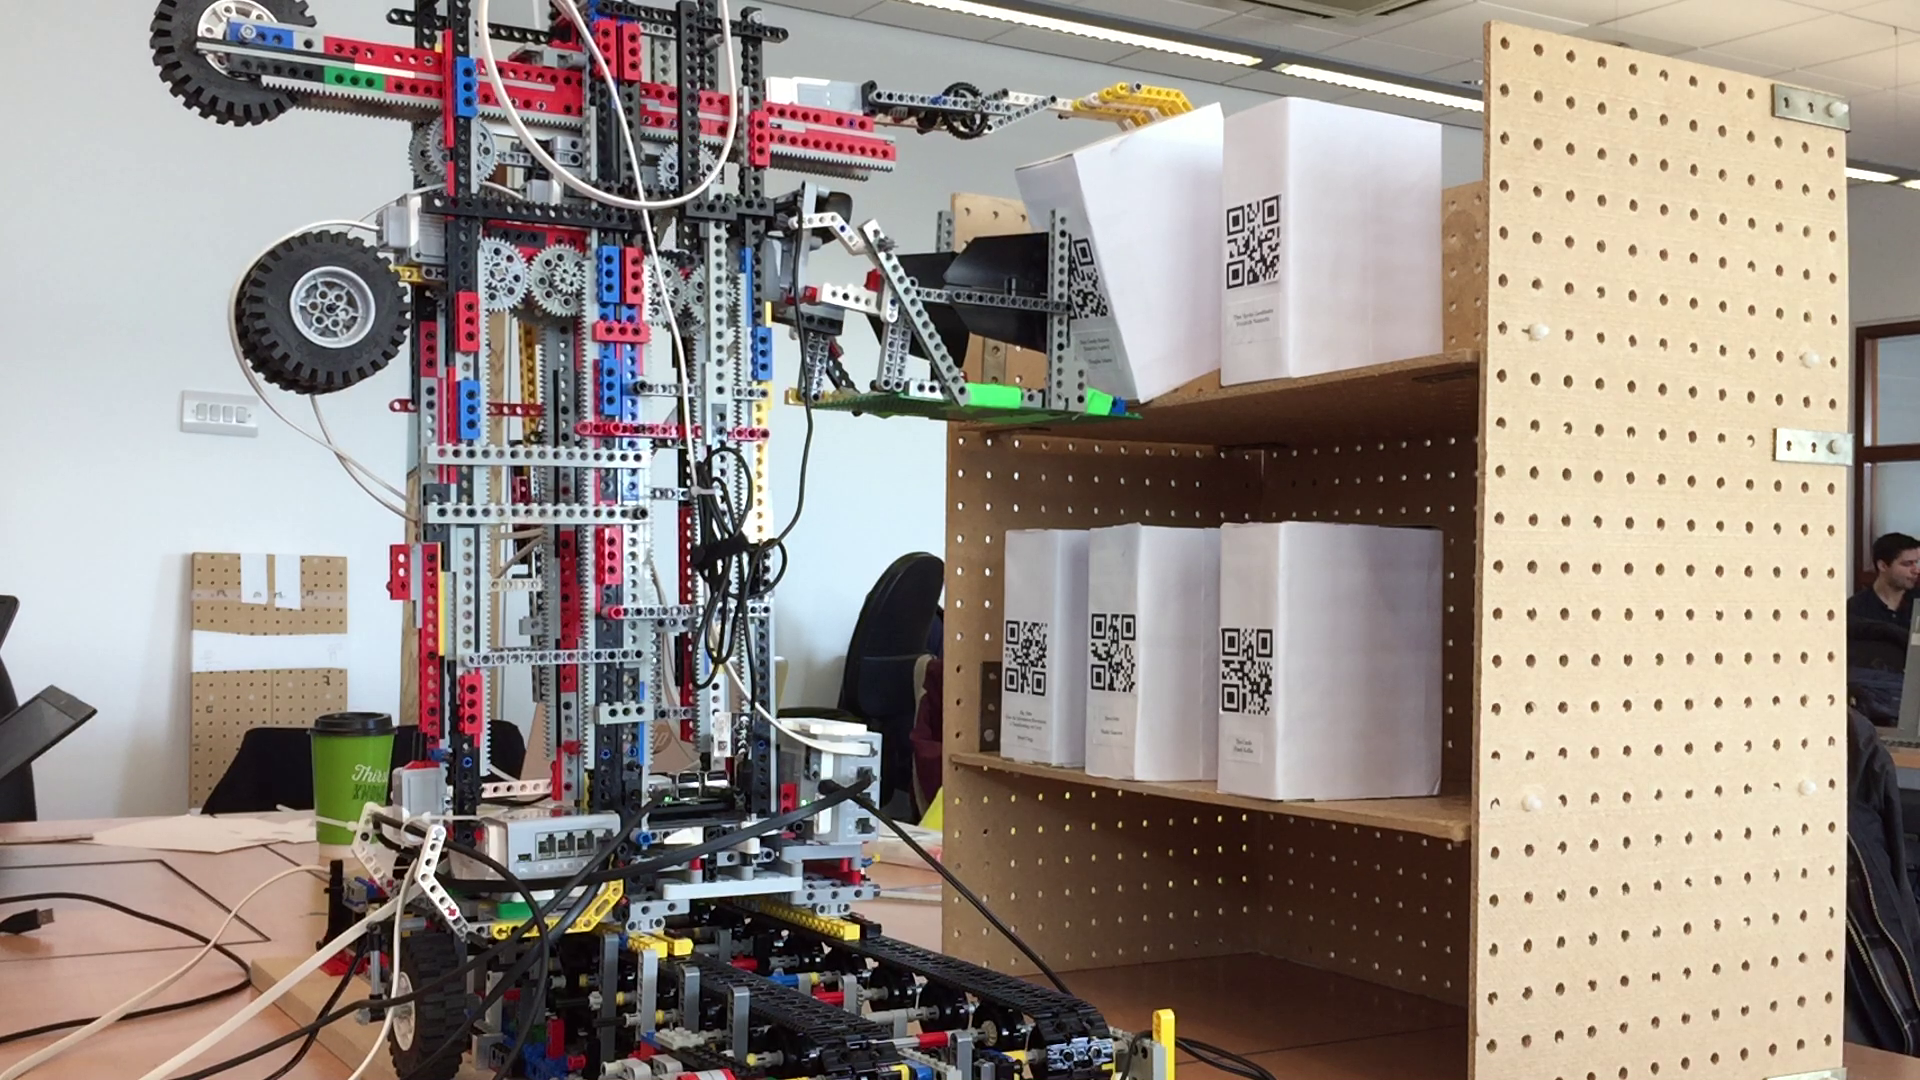
\includegraphics[width=\columnwidth]{figs/crane}}
%\caption{Lego construction: highlight any salient features in the caption}
%\label{fig:sample-fig}
%\end{center}
%\vskip -5mm
%\end{figure} 

\subsection{User interface}

Depending on your system and its stage of development, it could be useful to include a section about the user interface design, and the usability decisions behind it. Note, however, that you will be asked to provide a separate 'user guide' for the final demo.

\subsection{Software}

%Explain the key details of the control and interface software developed for the project. Be clear about any packages used and the reason for choosing them. 

%If you present algorithms, you can use the \verb+algorithm+ and \verb+algorithmic+ environments to format pseudocode (for instance, Algorithm~\ref{alg:example}). These require the corresponding style files, \verb+algorithm.sty+ and \verb+algorithmic.sty+ which are supplied with this package. 

TurtleBot movement is currently using a method based upon predefined paths which it is able to follow.
We have created a series of functions which can make the TurtleBot move in either a straight line for a given distance or rotate by a given angle.
To ensure that the TurtleBot has executed the move correctly we are using optometry data to determine when the move has been completed. 
To gather odometer feedback we are using the ROS odom topic, as this has already been implemented for the TurtleBot and has so far proved fairly accurate.
In future we will use the TurtleBots measured speed and LIDAR data to increase accuracy.
We are currently using predefined paths to allow us to test that the movement of the TurtleBot is working as expected. In future we expect to be able to generate these paths based on a predefined map, and a given start and finish location.

We considered using the ROS navigation stack, however it was proving difficult to implement due to a lack of the control software on DICE and missing libraries on the TurtleBot. 
Based on this, and the advice of one of the SDP experts we have decided to use our own navigation implementation.

\section{Evaluation}

We tested our hardware subsystem by repeatedly lifting a static load on the forklift to test reliability. As the forklift is currently a demo out of LEGO, testing was not intensive and we didn't calculate the max load bearing.
Software was tested by having an Android app emulator activate a script on the TurtleBot while both were connected to the "SDProbots" network.

\begin{table}[h]
    \vskip 3mm
    \begin{center}
    \begin{small}
    \begin{sc}
    \begin{tabular}{lcccr}
    \hline
    \abovespace\belowspace
    Test  & Time(mins) & Errors & Success \\
    \hline
    \abovespace
    1    & 0:06 & 0 & $\surd$ \\
    2    & 0:06 & 0 & $\surd$\\
    3    & 0:06 & 0 & $\surd$ \\
    4    & 0:06 & 0 & $\surd$\\
    5    & 0:06 & 0 & $\surd$ \\
    \hline
    \end{tabular}
    \end{sc}
    \end{small}
    \caption{Results for 5 tests on forklift movement with fixed light load.}
    \label{tab:sample-table}
    \end{center}
    \vskip -3mm
\end{table}

\begin{table}[h]
    \vskip 3mm
    \begin{center}
    \begin{small}
    \begin{sc}
    \begin{tabular}{lcccr}
    \hline
    \abovespace\belowspace
    Test  & Time(mins) & Errors & Success \\
    \hline
    1    & 0:06 & 0 & $\surd$ \\
    2    & 0:07 & 0 & $\surd$\\
    3    & 0:06 & 0 & $\surd$ \\
    4    & 0:06 & 0 & $\surd$\\
    5    & 0:06 & 0 & $\surd$\\
    6    & 0:06 & 0 & $\surd$ \\
    \hline
    \end{tabular}
    \end{sc}
    \end{small}
    \caption{Results for 6 tests on app communication with TurtleBot.}
    \label{tab:sample-table}
    \end{center}
    \vskip -3mm
\end{table}

\section{Budget}
Each report should contain an actualization of the estimated total budget 
of your system.


%submit sdp CDemX [filename] 

%where \verb|X| is the number of the demonstration (between 1 and 4) and \verb|[filename]| is the name of your file. The filename must be  \verb|group-[g]-demoX.pdf| where \verb|[g]| is the group number and again  \verb|X| is the demo number.
%This document should be submitted by a group member nominated for this purpose, and also emailed to the group mentor and to the TA at the time of submission.

%where \verb|[filename]| is the name of your user guide file. The filename must be  \verb|group-[g]-userguide.pdf| where \verb|[g]| is the group number.


%% Include any references in a bibliography

\bibliography{example-refs}

\end{document} 

